\documentclass[../../ASSD_TP1_G7.tex]{subfiles}
\begin{document}
\chapter*{Muestreo sub-Nyquist}
El muestreo sub-Nyquist se utiliza para se\~nales acotadas en banda con el espectro fuera de la Banda base. Para analizar este tipo de muestreo se utilizo una se\~nal AM, ya que su espectro coincide con las característica deseada.
\begin{equation}
X_c=A_{Max}[\frac{1}{2}cos(2\pi (1.8 f_{in})t)+cos(2\pi (2 f_{in})t)+cos(2\pi (2.2 f_{in})t)]
\end{equation}\label{eq:inputSignlan}

Donde $f_{in}= 36KHz$, entonces la frecuencia de la portadora es $72KHz$ y la modulada $7.2KHz$.
\section*{Rango de frecuencia de sampleo}
Definiendo $B$ al ancho de banda de la se\~nal y $f_c$ a la frecuencia central del espectro. El rango de frecuencias de sampleo $(f_s)$ es:
\begin{equation}
f_{sMIN}=\frac{2f_c + B}{m+1} < \frac{2f_c - B}{m} = f_{sMAX}
\end{equation}
Donde $m$ son las repeticiones del espectro. Conociendo $f_{in}$ y la se\~nal AM, $B=14.4KHz$ y $f_c=72KHz$.

\begin{table}[htbp]
\begin{center}
\begin{tabular}{|l|l|l|}
\hline
$m$ & $f_{sMIN}$ & $f_{sMAX}$  \\
\hline \hline
2 & $52.8KHz$ & $64.8KHz$ \\ \hline
3 & $39.6KHz$ & $43.2KHz$ \\ \hline
4 & $31.7KHz$ & $32.4KHz$ \\ \hline
\end{tabular}
\caption{Frecuencias de Sampleo}
\label{tabla:fsamp}
\end{center}
\end{table}
Para $m$ mayores, $f_{sMIN}>f_{sMAX}$.
\section*{Mediciones}
Las mediciones se realizaron para el caso de $m=2$.
\subsection*{Llave Analógica}

\begin{figure}[H]
\centering
\subcaptionbox{Simulación}
{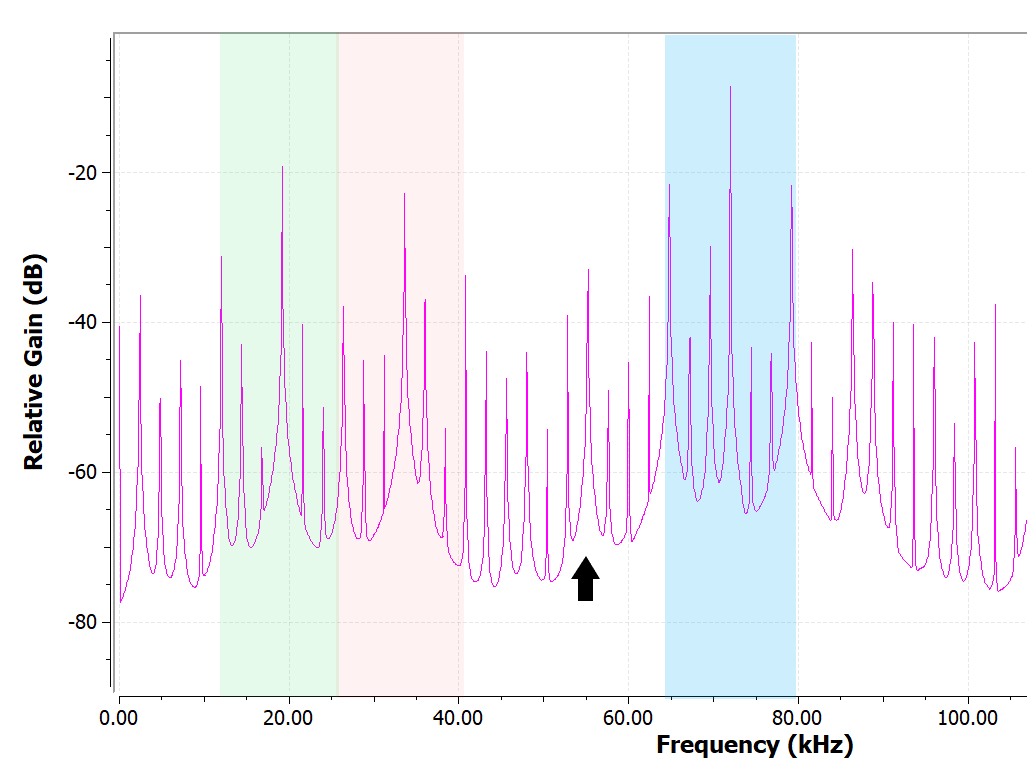
\includegraphics[width=0.45\textwidth]{figures/simpto_8_llave_52,8khz_espectro.png}}
\subcaptionbox{Medición}
{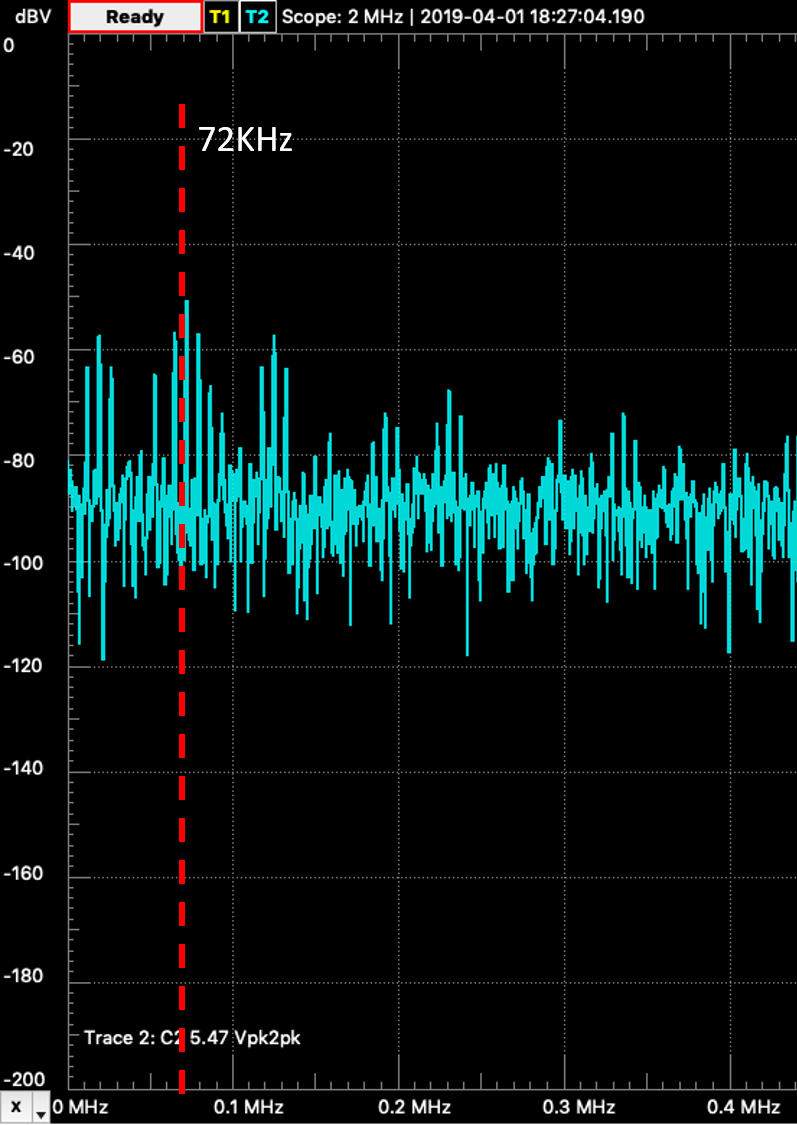
\includegraphics[width=0.45\textwidth]{figures/pto_8_llave_52,8khz_espectro.png}}
\caption{Frecuencia sampleo mínima(52.8KHz), simulación y medición}
\end{figure}

\begin{figure}[H]
\centering
\subcaptionbox{Simulacion}
{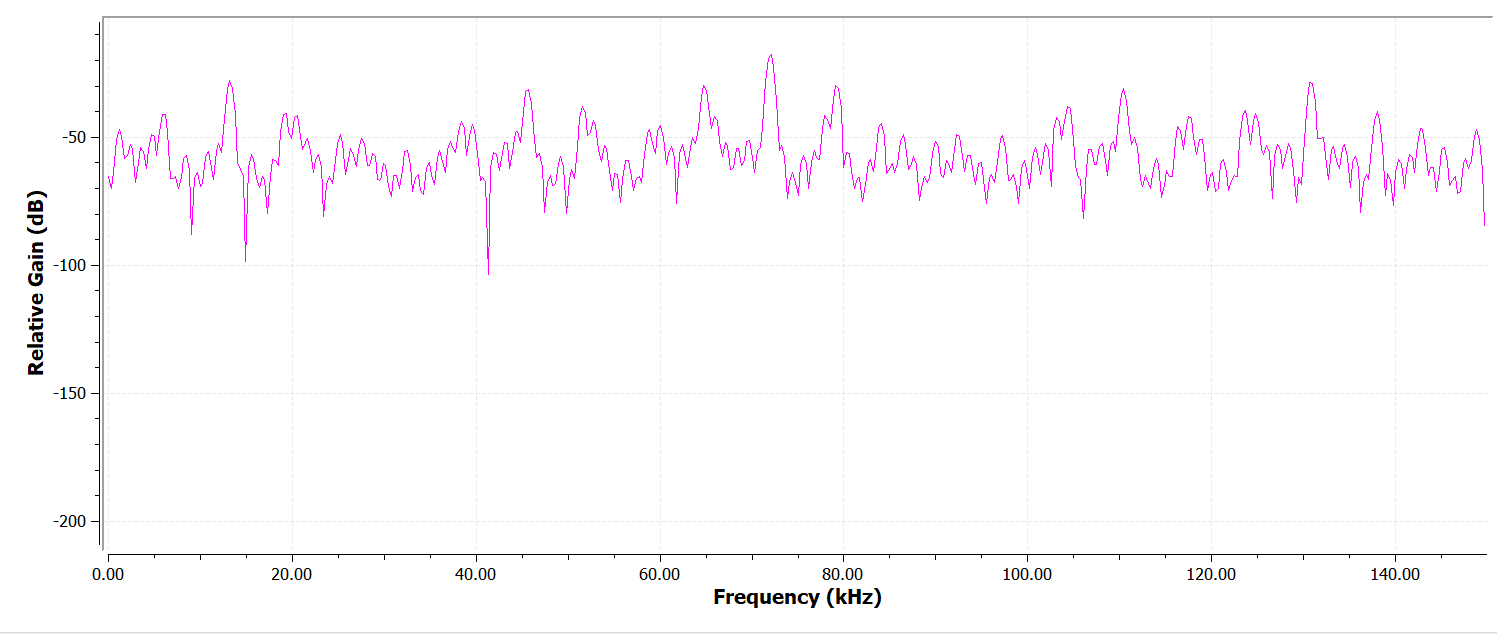
\includegraphics[width=0.45\textwidth]{figures/simpto_8_llave_58,8_espectro.png}}
\subcaptionbox{Medicion}
{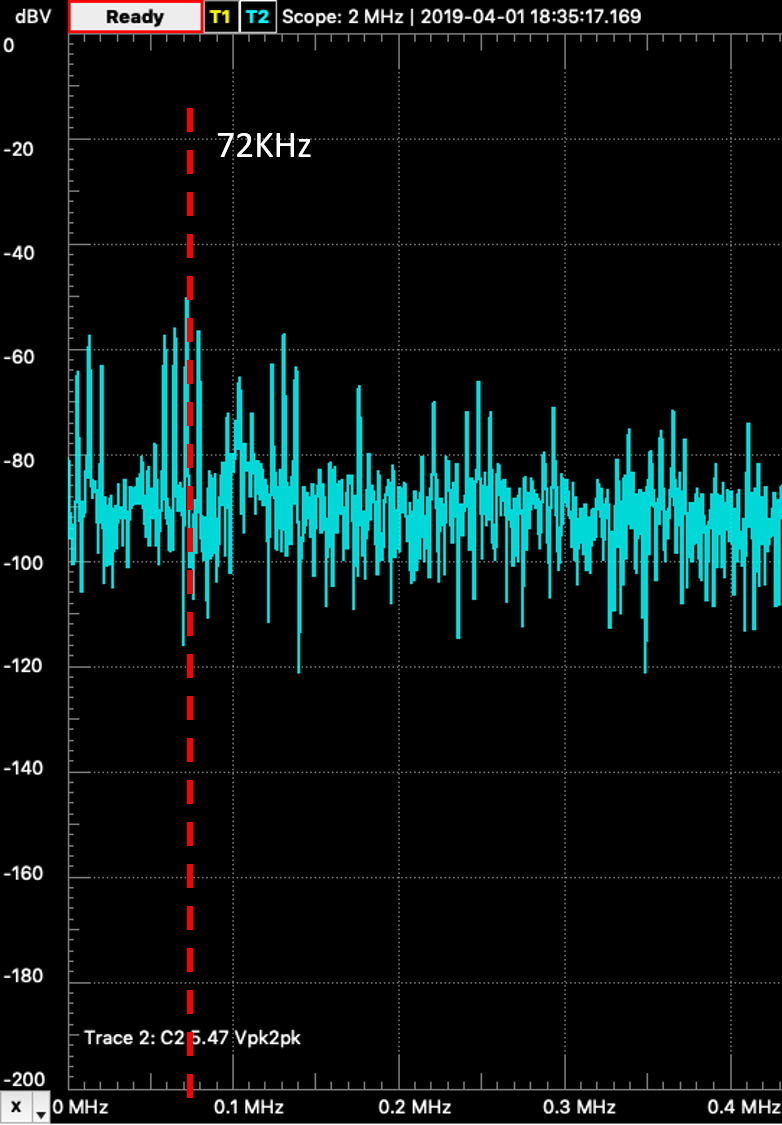
\includegraphics[width=0.45\textwidth]{figures/pto_8_llave_58,8_espectro.png}}
\caption{Frecuencia sampleo media(58.8KHz), simulación y medición}
\end{figure}

\begin{figure}[H]
\centering
\subcaptionbox{Simulación}
{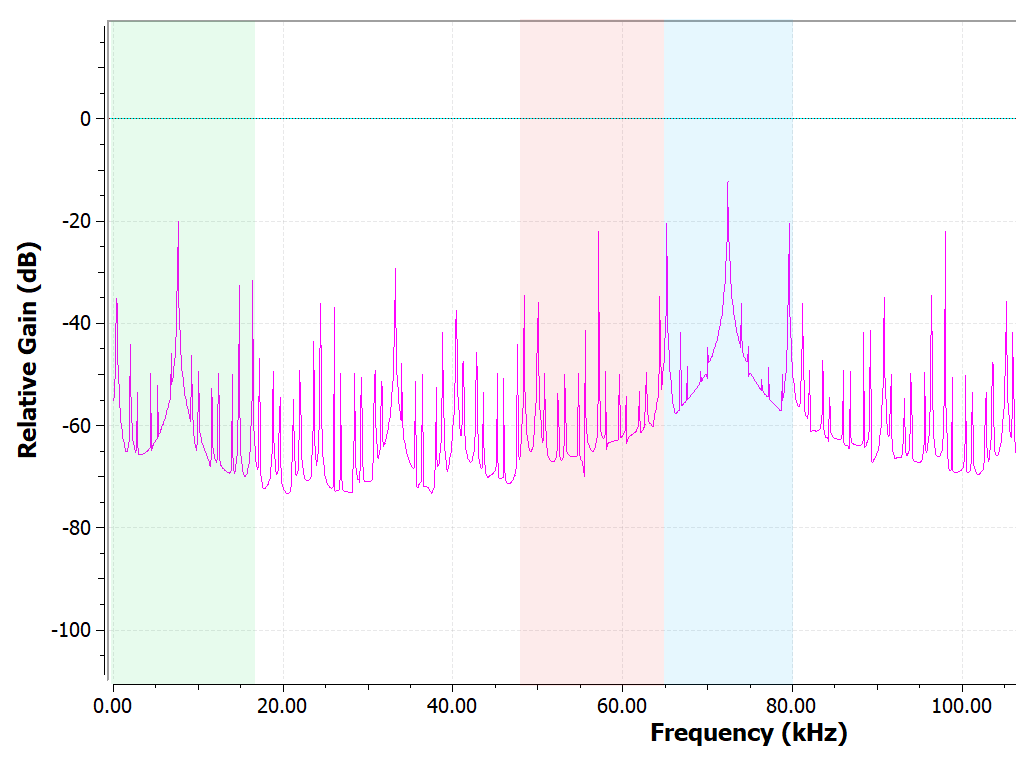
\includegraphics[width=0.45\textwidth]{figures/simpto_8_llave_64,8khz_espectro.png}}
\subcaptionbox{Medición}
{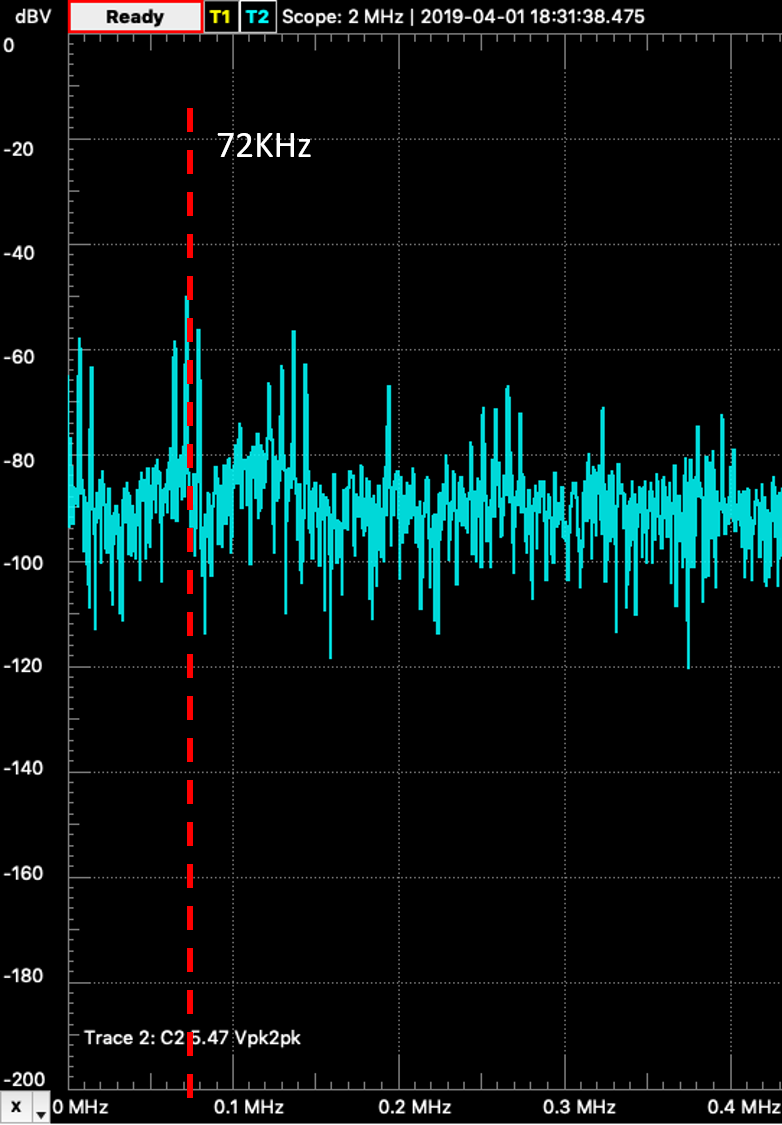
\includegraphics[width=0.45\textwidth]{figures/pto_8_llave_64,8khz_espectro.png}}
\caption{Frecuencia sampleo maxima(64.8KHz), simulación y medición}
\end{figure}


\subsection*{Sample and Hold}


\begin{figure}[H]
\centering
\subcaptionbox{Simulación}
{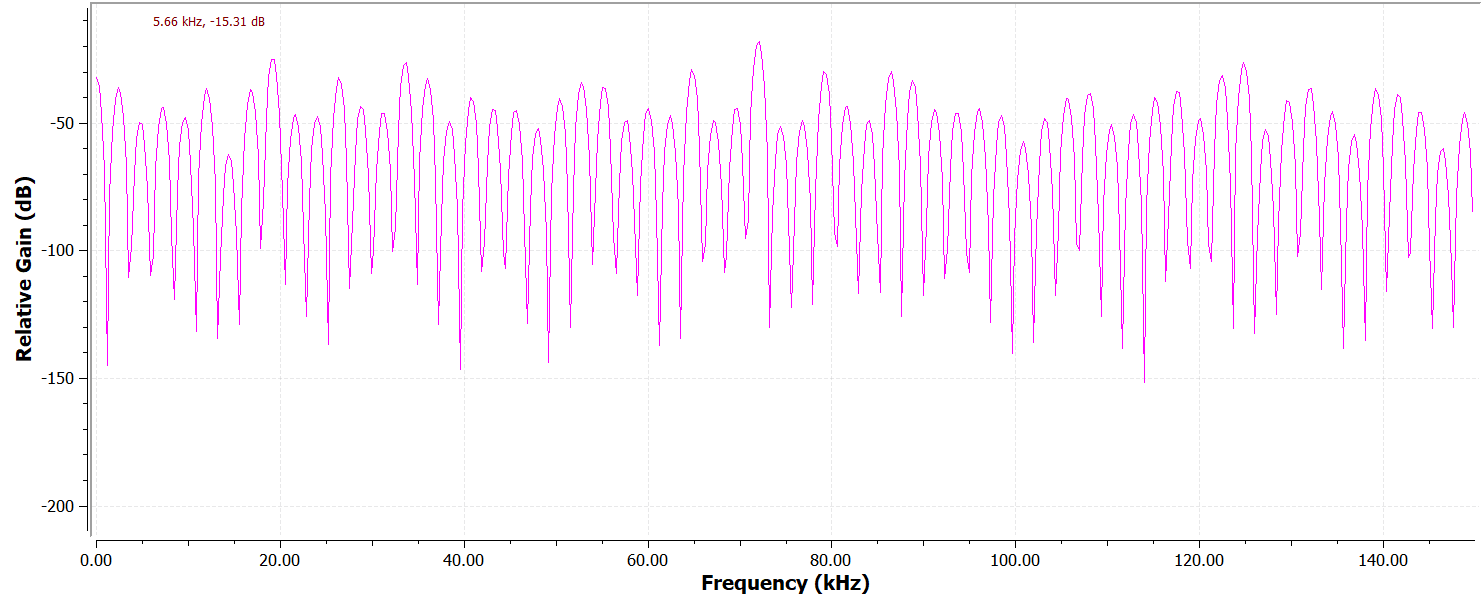
\includegraphics[width=0.45\textwidth]{figures/simpto_8_syh_52,8_espectro.png}}
\subcaptionbox{Medición}
{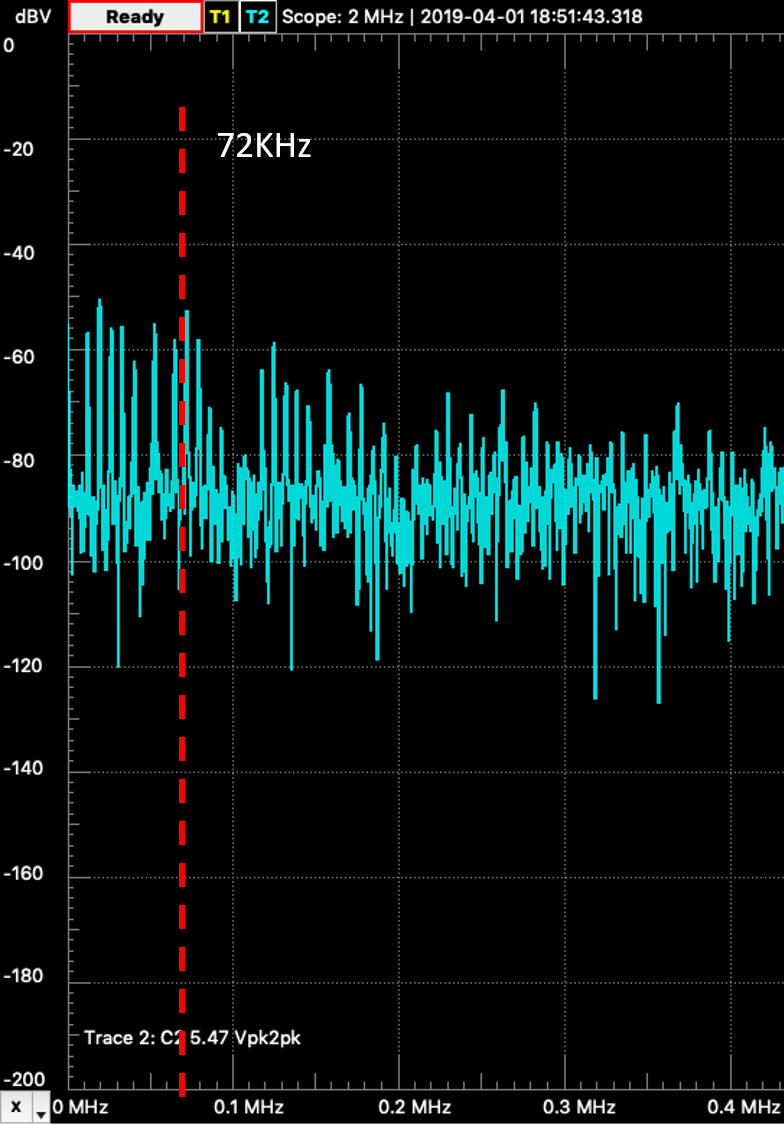
\includegraphics[width=0.45\textwidth]{figures/pto_8_syh_52,8_espectro.png}}
\caption{Frecuencia sampleo mínima(52.8KHz), simulación y medición}
\end{figure}

\begin{figure}[H]
\centering
\subcaptionbox{Simulacion}
{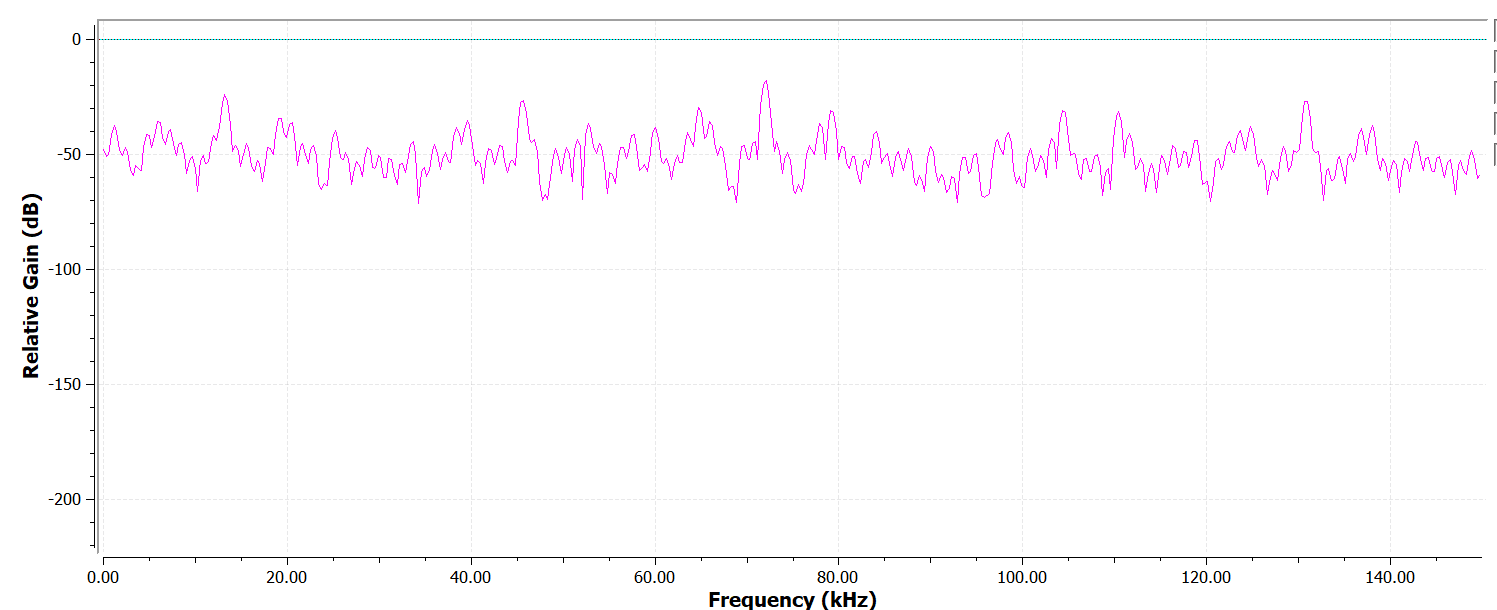
\includegraphics[width=0.45\textwidth]{figures/simpto_8_syh_58,8_espectro.png}}
\subcaptionbox{Medicion}
{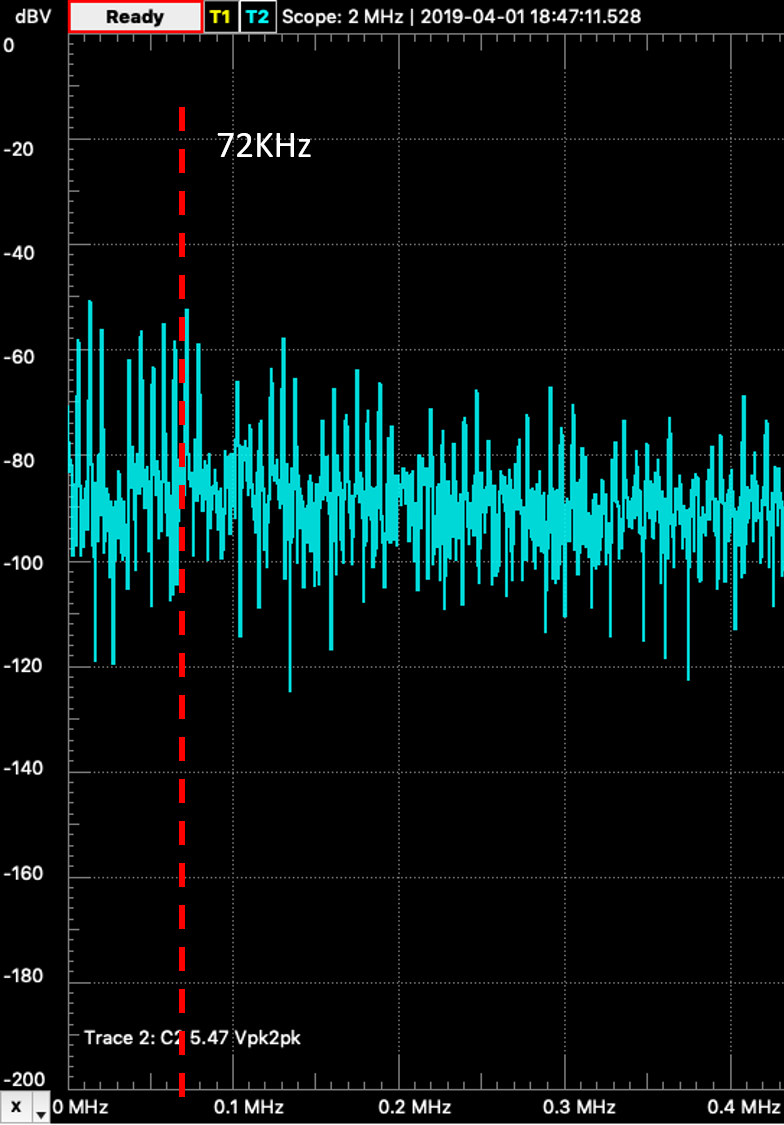
\includegraphics[width=0.45\textwidth]{figures/pto_8_syh_58,8_espectro.png}}
\caption{Frecuencia sampleo media(58.8KHz), simulación y medición}
\end{figure}

\begin{figure}[H]
\centering
\subcaptionbox{Simulación}
{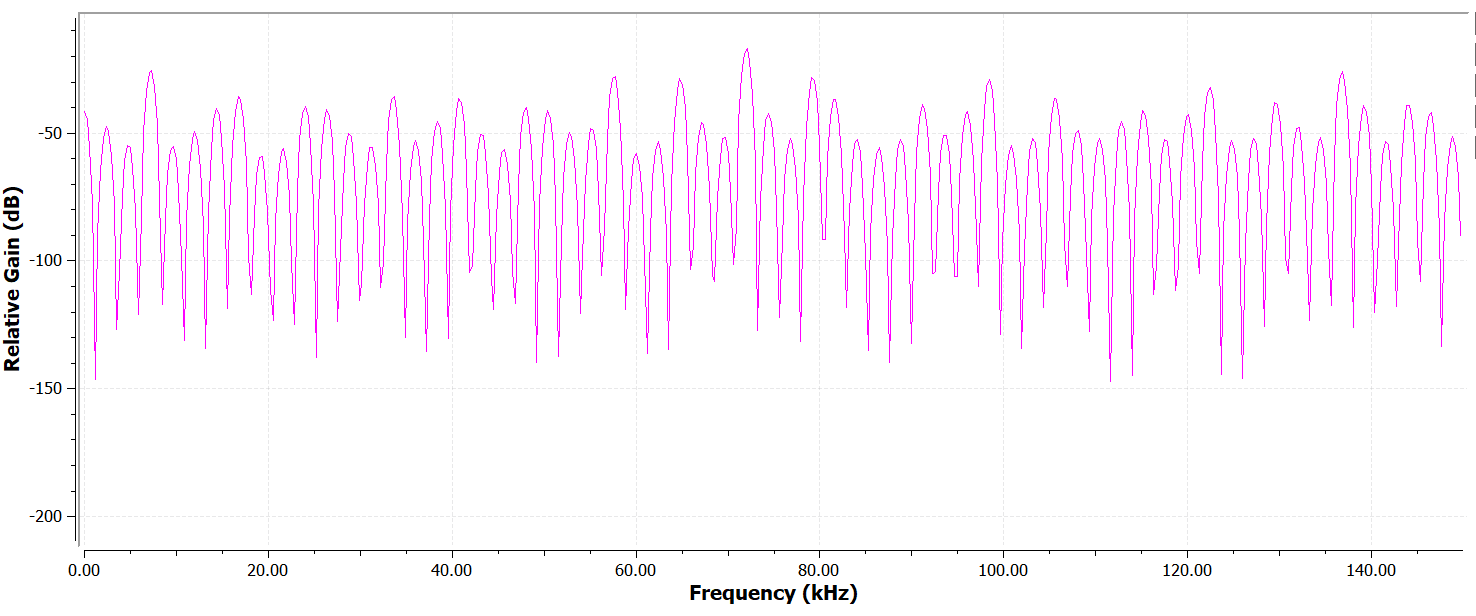
\includegraphics[width=0.45\textwidth]{figures/simpto_8_syh_64,8_espectro.png}}
\subcaptionbox{Medición}
{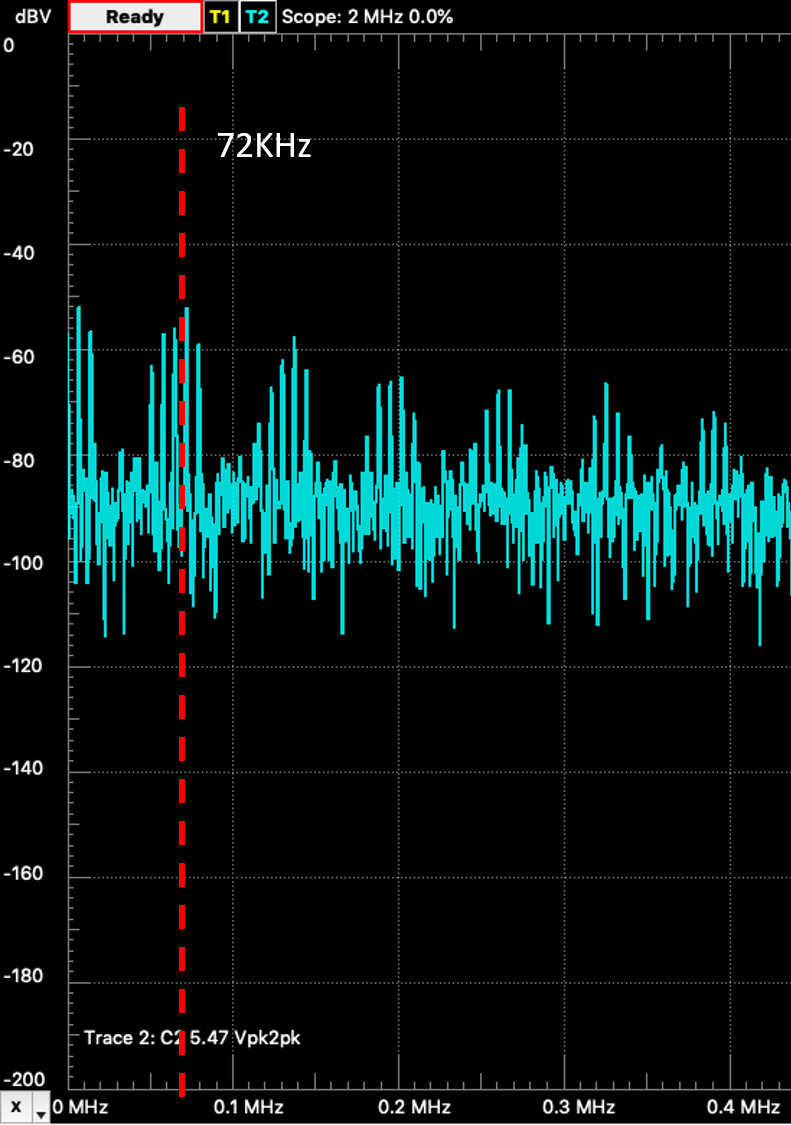
\includegraphics[width=0.45\textwidth]{figures/pto_8_syh_64,8_espectro.png}}
\caption{Frecuencia sampleo maxima(64.8KHz), simulación y medición}
\end{figure}




\end{document}
